It was right around the year in which I was born that the American political economist Francis Fukuyama captured the mood of much of the world by claiming that history was ending\cite{Fukuyama1992}. This feeling was based on the fall of the Berlin wall and with it what seemed like the inevitable spread to the entire world of societal structures and lifestyles based on inclusive liberal democracy, technological progress, and market capitalism tempered to varying extent by regulatory welfare states. Now, a widely accepted view that history was ending seems itself to be part of a rather brief moment in history, shattered 
%in part by wars and revolutions that broadly failed in their (generously interpreted) intentions of spreading democracy, the astounding success (in some respects) of China's politically authoritarian societal model, and a growth of illiberal political views in established democracies. 
by several waves of headline-dominating setbacks to the advancement of these supposedly victorious ideals.
But nothing poses a more devastating blow to the supposed inevitability of our lifestyles and societies than does the fact that they are simply unsustainable. History is not over, because if we try to keep on living the way we do today, we won't be able to keep living on this planet.

\begin{figure}[h!]
	\centering
	\includegraphics[width=0.7\textwidth]{01_Intro/fig/carbon_cycle.png}
	\caption{Diagram of Earth's carbon cycle. Red numbers indicate the fluxes and accumulations associated with the anthropogenic perturbation. From ref. \citen{DOE2008}, based on data from ref. \citen{LeQuere2015}}
	\label{fig:carbon_cycle}
\end{figure}

The un-sustainability of humanity in its present state encompasses the crossing of multiple planetary boundaries\cite{Rockstrom2009}, but none pose a more existentially urgent challenge to human civilization than climate change. The root of our problem, as we summarize it in the introduction to Paper \ref{Nitopi2019}, is that:

\begin{quotation}
		{\Large``} At the core of biological metabolism is the ability to convert carbon between different oxidation states in order to store and release energy, as well as to synthesize functional molecules. Likewise, the oxidation of carbon is at the center of human civilization's collective “industrial metabolism” consisting of our energy infrastructure and chemical industry. Whereas in biological metabolism, reduction of \ch{CO2} in photosynthesis balances the oxidation of carbon in cellular respiration, carbon reduction is as of yet a missing piece of humanity's industrial metabolism. This imbalance has become a significant perturbation to Earth’s natural carbon cycle... The resulting accumulation of the greenhouse gas \ch{CO2} in the atmosphere is the primary	driver of today’s climate change\cite{IPCC2014}. {\Large''}
\end{quotation}

This imbalance is illustrated in Figure \ref{fig:carbon_cycle} and in Table 1 of Paper \ref{Nitopi2019}. So far, since humans began burning fossil fuels at scale in the 1800's, we have moved approximately 400 gigatons of carbon (GtC) from the ground to the air as carbon dioxide (\ch{CO2}), about half of which has stayed in the atmosphere, increasing the atmospheric \ch{CO2} concentration from less than 300 ppm to more than 400 ppm\cite{IPCC2014, LeQuere2018}. At the writing of this Thesis, the atmospheric \ch{CO2} concentration was 412 ppm and increasing at an annualized rate of about 3 ppm per year\cite{NOAA2019}. 

\begin{figure}[h!]
	\centering
	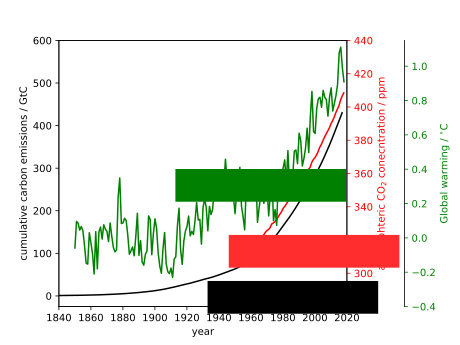
\includegraphics[width=0.7\textwidth]{01_Intro/fig/global_warming.png}
	\caption{Cumulative carbon emissions (black), atmospheric \ch{CO2} concentration (red), and global mean surface temperature relative to the 1850-1900 average (green). Made with data from refs. \citen{LeQuere2018}, \citen{Morice2012}, and \citen{Ritchie2019a}.}
	\label{fig:temperatures}
\end{figure}

Climate science is beyond the scope of this Thesis, but, in brief: \ch{CO2} and other greenhouse gases absorb infrared radiation, unlike the primary components of the atmosphere \ch{N2} and \ch{O2}. Infrared radiation is the main way earth sheds heat to space to balance all the energy coming in as sunlight, so \ch{CO2} in the atmosphere acts like a blanket, heating up the earth. This has so far resulted in an increase in the average temperature of the earth's surface of about 1$^\circ$ C, as shown in Figure \ref{fig:temperatures}. An increase in the average temperature of the earth is worse than it might sound, because the extra energy that this represents effects the entire climate system in profound ways. Climate change is increasing the intensity and frequency of all kinds of extreme weather events including heat waves, forest fires, floods, storms, and droughts\cite{IPCC2014, CarbonBrief}. 
\begin{figure}[h!]
	\centering
	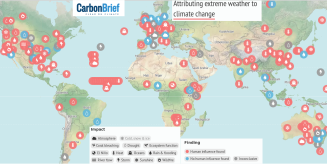
\includegraphics[width=\textwidth]{01_Intro/fig/climate_change_effects.png}
	\caption{Map of recent extreme weather events from 2011 to 2018. Red indicates that the risk of the extreme weather event was increased by climate change. From %\url{https://www.carbonbrief.org/mapped-how-climate-change-affects-extreme-weather-around-the-world}.
	ref \citen{CarbonBrief}.
}
	\label{fig:attribution}
\end{figure}

Weather is naturally variable, but the science of \textit{climate attribution} has progressed in recent years. Now, the increase in the likelihood due to climate change of a given extreme weather event can be readily calculated, giving a clear picture of the worsening adverse effects of our emissions\cite{Schiermeier2018}. Figure \ref{fig:attribution}, from ref. \citen{CarbonBrief}, shows a map of recent extreme weather events, many of which are attributed to climate change. Extreme weather events and natural disasters are deadly even in developed countries with strong states. In developing countries they can destabilize societies and displace millions. The frequency and severity of climate-change-related extreme weather events will worsen significantly if the present warming trend is not stopped\cite{IPCC2018_SPM}. 

Fortunately for those of us who broadly like living under or aspire to live under enlightenment ideals (and for Fukuyama's assertion), there is still reason to hope that the worst possible outcomes of climate change can be averted within the frameworks of liberal democracy and regulated market capitalism. However, this will not be easy. It will require far-sightedness on the part of both leaders and everyone who chooses them. It will require unprecedented willpower from many corners of society. We will almost certainly need to change our lifestyles significantly, and we will with complete certainty have to change the way we power our lives entirely. 

The scale and scope of these required changes, both societal and technological, is outlined (very briefly) in the first Section of this Chapter. The second Section describes a central component to the required technological changes: a growing role for electrochemistry in decarbonizing energy, transport, and industry. This will motivate Chapters \ref{ch:Tools} and \ref{ch:Oxygen}, which describe methods and results in fundamental electrocatalysis studies which will hopefully contribute to breakthroughs accelerating electrochemistry's growing role. Finally, in \ref{ch:Impact}, the Thesis ties these results back to the climate crisis by estimating the net \ch{CO2} impact (emitted minus saved) resulting from this PhD project.
